
\section{Diagnosis en \\ Hematología/Oncología}
La Hematología/Oncología es la rama de la medicina que se centra en el diagnóstico y tratamiento de numerosos trastornos sanguíneos, incluidos el cáncer, la anemia, la leucemia y la enfermedad de Hodgkin, y el diagnóstico y tratamiento de cánceres y tumores benignos y malignos.

La mejor manera de detectar el melanoma es examinando continuamente la piel de los pacientes, especialmente los lunares. Una llaga, una protuberancia o un tumor en la piel también puede ser un signo de melanoma u otro cáncer de piel. El melanoma se puede encontrar en varios lugares incluyendo la espalda, las nalgas, las piernas, el cuero cabelludo, el cuello, detrás de la oreja, las plantas de los pies, las palmas de las manos, dentro de la boca, los genitales y debajo de las uñas. 

Según la Academia Americana de Dermatología (AAD), aproximadamente del 20\% al 40\% de los melanomas se desarrollan a partir de un lunar. Una llaga o tumor que sangra o cambios en el color de la piel también puede ser un signo de cáncer de piel. 

\pagestyle{fancy}
\fancyhf{}
\fancyhead[L]{2. DIAGNOSIS EN HEMATOLOGÍA/ONCOLOGÍA}
La clave para tratar con éxito el melanoma es reconocer los síntomas a tiempo. Se recomienda realizar exámenes corporales anuales por un dermatólogo y examinarse la piel una vez al mes. Si un paciente ha tenido cáncer de piel, debe hacerse chequeos regulares para que un médico pueda examinar su piel.
Hay un número de pruebas que se pueden ordenar para diagnosticar el cáncer de piel: 
\begin{itemize}
\item Biopsia
\item Tomografía computarizada (TC)
\item Imagen de resonancia magnética (IRM)
\item Tomografía por emisión de positrones (TEP)
\end{itemize}
Por lo que un clasificador que sea capaz de discernir entre imágenes de piel de cáncer maligno y benigno ayudaría al diagnóstico mensual que deben hacer los médicos a sus pacientes además de reconocer los síntomas a tiempo.
\newpage

\pagestyle{fancy}
\fancyhf{}
\fancyhead[L]{2.1 CONJUNTO DE DATOS}

\subsection{Conjunto de datos}
Para crear un modelo que sea capaz de clasificar las imágenes de cáncer se ha hecho uso de un conjunto de datos generado por la International Skin Imaging Collaboration (ISIC) en en donde las imágenes provienen de las siguientes fuentes: Hospital Clínic de Barcelona, Medical University of Vienna, Memorial Sloan Kettering Cancer Center, Melanoma Institute Australia, University of Queensland y University of Athens Escuela de Medicina.
\bigskip

Este conjunto de datos contiene 33.126 imágenes de entrenamiento dermatoscópicas de lesiones cutáneas benignas y malignas únicas de más de 2.000 pacientes. Cada imagen se asocia con una de estas personas mediante un identificador de paciente único. Todos los diagnósticos malignos se han confirmado mediante histopatología, y los diagnósticos benignos se han confirmado mediante el acuerdo de expertos, el seguimiento longitudinal o la histopatología. 
\bigskip

El conjunto de datos fue seleccionado para el SIIM-ISIC Melanoma Classification Challenge organizado en Kaggle durante el verano de 2020.
\bigskip

\newpage
\pagestyle{fancy}
\fancyhf{}
\fancyhead[L]{2.2 PREPROCESAMIENTO DE DATOS}

\subsection{Exploración de datos}
==$>$ Escribe sobre el preprocesamiento (desequilibrado, tipo de red que se va a usar…).

\begin{figure}[htbp]
    \centering
    \textbf{}\par\medskip
    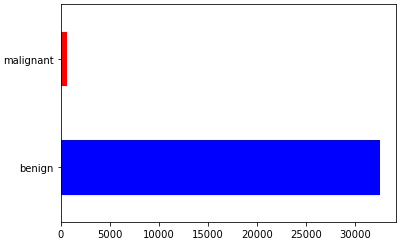
\includegraphics[scale=0.90]{figures/metadata/imbalance_class.PNG}
    \caption{Desequilibrio de clases}
\end{figure}

\begin{center}
\begin{tabularx}{0.5\textwidth} { 
  | >{\centering\arraybackslash}X 
  | >{\centering\arraybackslash}X |}
 \hline
 Tipo & Total de muestras  \\
 \hline
 benign & 32542 \\
 \hline
 malignant & 584 \\
 \hline
\end{tabularx}
\end{center}

\begin{figure}[htbp]
    \centering
    \textbf{}\par\medskip
    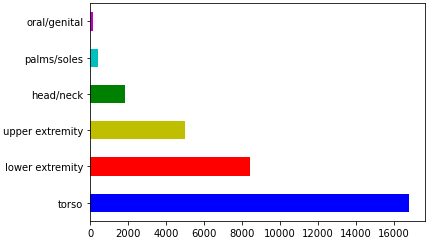
\includegraphics[scale=0.90]{figures/metadata/anatom_site_general_count.PNG}
    \caption{Parte del cuerpo}
\end{figure}

\begin{figure}[htbp]
    \centering
    \textbf{}\par\medskip
    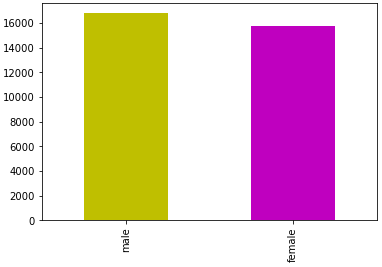
\includegraphics[scale=0.90]{figures/metadata/gender_count.PNG}
    \caption{Recuento de género}
\end{figure}

\begin{figure}[htbp]
    \centering
    \textbf{}\par\medskip
    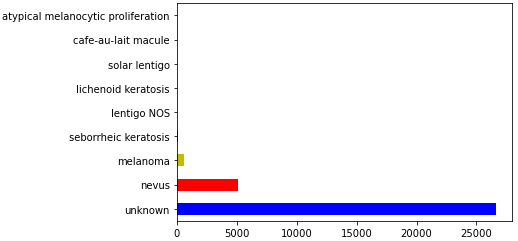
\includegraphics[scale=0.90]{figures/metadata/diagnosis_count.PNG}
    \caption{Diagnóstico}
\end{figure}

\begin{figure}[htbp]
    \centering
    \textbf{}\par\medskip
    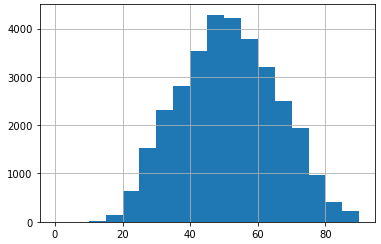
\includegraphics[scale=0.90]{figures/metadata/age_count.PNG}
    \caption{Recuento de edades}
\end{figure}